\documentclass{article}
\usepackage[utf8]{inputenc}
\usepackage{titling}
\usepackage{graphicx}
\usepackage{xcolor}
\usepackage[colorlinks=true,linkcolor=darkgray, urlcolor =gray]{hyperref}
\usepackage[spanish]{babel}
\DeclareUnicodeCharacter{301}{~}
\usepackage{url}


\title{Práctica 3. Modelos canónicos y su implementación en GeNIe}
\author{Cristina Díaz García}
\date{Marzo 2019}

\renewcommand\maketitlehooka{\null\mbox{}\vfill}
\renewcommand\maketitlehookd{\vfill\null}


\begin{document}

\addcontentsline{toc}{section}{Índice general}

\begin{titlingpage}
\maketitle
\end{titlingpage}

\newpage

\tableofcontents

\newpage

\section{Enunciado}

\textbf{\underline{Tarea:}} Implementa en GeNIe una puerta OR en la que haya tres causas y un efecto. Razona la forma de construir la CPT en este caso (fórmula). Comprueba \underline{para un par de casos} que los resultados coinciden con el cálculo que realiza GeNIe.

\textbf{\underline{Entrega:}} Sube un fichero pdf en el que incluyas captura de pantalla de tu red GeNIe y de las tres tablas de probabilidad mencionadas anteriormente (tablas 1, 2 y 3) y también la demostración de que la fórmula que has aplicado te da los resultados correctos (con un par de casos es suficiente).

\section{Modelado de la puerta OR}

\subsection{\textbf{Modelo}}

\begin{center}
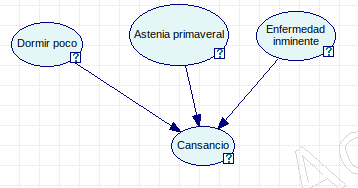
\includegraphics[scale=0.5]{modelo.png}
\end{center}

\subsection{\textbf{Tablas}}

\textbf{Tabla de probabilidades sin tener en cuenta el ruido:}

\begin{center}
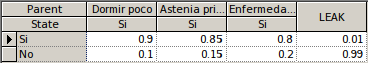
\includegraphics[scale=0.5]{tabla1.png}
\end{center}

\textbf{Tabla de probabilidades teniendo en cuenta el ruido:}

\begin{center}
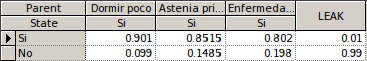
\includegraphics[scale=0.5]{tabla2.png}
\end{center}

\textbf{Tabla de probabilidad condicionada:}

\begin{center}
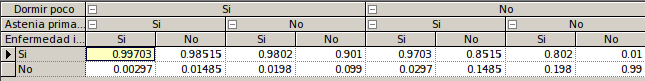
\includegraphics[scale=0.5]{tabla3.png}
\end{center}

\subsection{\textbf{Demostraciones}}

\begin{center}
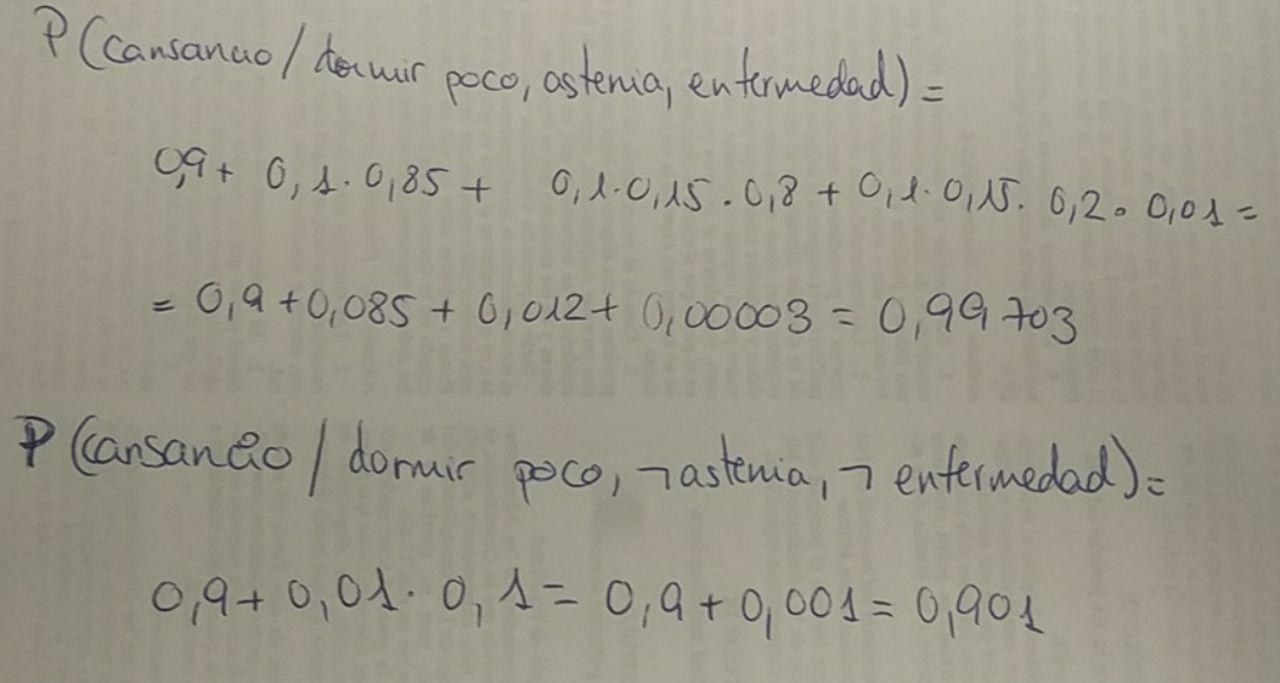
\includegraphics[scale=0.4]{demostraciones.jpg}
\end{center}

\section{Otros modelos canonicos}

\subsection{\textbf{Noisy-AND}}

\textbf{Modelo:}

\begin{center}
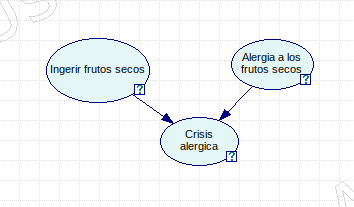
\includegraphics[scale=0.5]{and.png}
\end{center}

\textbf{Tabla de probabilidades sin tener en cuenta el ruido:}

\begin{center}
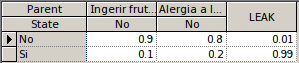
\includegraphics[scale=0.5]{and1.png}
\end{center}

\textbf{Tabla de probabilidades teniendo en cuenta el ruido:}

\begin{center}
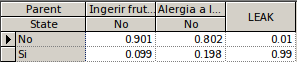
\includegraphics[scale=0.5]{and2.png}
\end{center}

\textbf{Tabla de probabilidad condicionada:}

\begin{center}
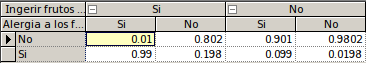
\includegraphics[scale=0.5]{and3.png}
\end{center}

\begin{thebibliography}{9}
\bibitem{Bayes} Información oficial de GeNIe, \url{https://www.bayesfusion.com}.
\end{thebibliography}

\end{document}